\documentclass[../main.tex]{subfiles}
\graphicspath{{\subfix{../img/}}}

\begin{document}

\subsection{Transition from Spiking to Bursting}

\subsubsection{EAG channel expression modulates spiking-bursting transition}

\noindent As it was discussed in Section \ref{subsubsec:transit_tonic_burst}, one possible mechanism behind the transition of R5 activity between tonic firing and bursting may be due to diurnal variation in expression of the \gls{eag} channel. \gls{eag} is permeable to potassium. During the night, expression of these channels is low compared to the day. %!TODO!: Citation
As potassium current is hyperpolarizing, increased expression of \gls{eag} channels during the day might potentially decrease excitability of the cell and thus, the number of spikes per burst.

\gls{eag} channels are voltage-gated ion channels. The family of \gls{eag} channels contains several subtypes. Some of them are inactivating (i.e. contain an inactivation gate), while others are non-inactivating (i.e. lack an inactivation gate) \parencite{bauerEtheragogoChannelsEffective2018}.
The kinetic properties of these channels in \textit{Drosophila} are not extensively documented in the literature. I could find only a single paper providing kinetic properties of these channels in \textit{Drosophila} \parencite{bronkRegulationEagCa22018}. Although the original model of the \gls{eag} channel described in the paper is blocked by Ca$^{2+}$, the present work assumes that the gating mechanism depends solely only on membrane potential, for simplicity. This simplification is justified for several reasons. First, the \gls{eag} channels are generally considered to be voltage-gated \cite{bauerEtheragogoChannelsEffective2018}. Second, to my knowledge, the exact biophysical properties of these channels have not been characterized in R5 neurons - only the expression of the gene encoding the channel has been identified in these cells \cite{doppSinglecellTranscriptomicsReveals2024}. Third, in the model proposed by Bronk and Schwarz, \gls{eag} channels are inactivated by calcium. However, for these channels to contribute to burst termination, the calcium-dependent inactivation must be either weak or sufficiently slow. Otherwise, calcium influx during a burst would prevent it from contributing to burst termination.
Therefore, calcium-dependent inactivation of \gls{eag} channels is unlikely to play a significant role in the transition from bursting to spiking in R5 neurons.

In the literature, bursting models generally lack \gls{eag} channels. Thus, I added the channel to the Wang model to test the above-mentioned hypothesis. The parameters for \gls{eag} channel were adapted from \parencite{bronkRegulationEagCa22018}, with few modifications that will be discussed below. The current through the channel \textcolor{red}{was added to the total ionic current} $\sum I_{\text{ion}}$ \textcolor{red}{in Equation ??? and is governed by}:
\begin{equation*}\label{eq:current_eag}
    I_{\text{EAG}} = g_{\text{EAG}} m^2 (V - V_K)
\end{equation*}
where $g_{\text{EAG}}$ is the conductance, $V_K$ is reversal potential of potassium, and $m$ is activation variable governed by Equation \ref{eq:differential_gating_steadyst_timeconst}. The voltage is measured in millivolts, while the maximal conductance and current are expressed in either $mS/cm^2$, or $S/cm^2$ and $\mu A/cm^2$ or $mA/cm^2$, respectively, depending on the model (Appendix \ref{appendix:functions_and_parameters}). The steady state activation $m_{\infty}(V)$, and activation time constant $\tau(V)$ are governed by:
\begin{equation}\label{eq:eag_steady_state_activation}
    m_\infty(V) = \left( \frac{1}{1 + \exp{(-(V+23.12-d)/k)}} \right)
\end{equation}
\begin{equation} \label{eq:eag_tau_activation}
    \tau(V) = a\left(5497 - \frac{5500}{1 + \exp( (V + 251.5 - d) / (-16.94-51.5) ) }\right)
\end{equation}
Note that Equation \ref{eq:eag_steady_state_activation} lacks dependency on calcium, in contrast to the one proposed in \parencite{bronkRegulationEagCa22018}. Equation \ref{eq:eag_steady_state_activation}, is a sigmoid function, where the parameter $k$ determines the slope of the sigmoid and was set to $16.94$ in \parencite{bronkRegulationEagCa22018}. 
The parameter $d$, measured in millivolts, was introduced into the model to allow a voltage shift in the steady-state activation function  $m_\infty(V)$ and the gating time constant $\tau(V)$. Since different models operate over slightly different membrane potential ranges, $d$ serves to adjust the voltage range in which the ion channel is active.
The parameter $a$, which is unitless, was introduced to scale the activation time constant. It modulates the rate at which the gating variable converges to its steady-state value at a given membrane potential.

To investigate whether the \gls{eag} channel can affect the number of spikes per burst, the parameters $d$ and $a$ were manually tuned such that the addition of the channel did not alter the oscillation period. This constraint was particularly important for the Wang model, as it is fragile with respect to perturbations in external current - small changes in input dramatically affect the oscillation period \cite{wangMultipleDynamicalModes1994}.
\textcolor{red}{In contrast, the Goldman model has been reported to be more robust to parameter variations due to the geometry of its nullclines \parencite{franciRobustTunableBursting2018}.}
In general, if the added ion channel conducts current at membrane potentials between bursts, the hyperpolarizing nature of the \gls{eag} current can counteract the depolarizing currents and delay the membrane potential from reaching the spiking threshold, thereby extending the oscillation period.

Note that this is a strong condition, motivated by literature reporting tonic firing of R5 neurons during the daytime.  However, further data analysis is needed, and it is possible that the assumption of tonic firing - and thus the above-mentioned requirement - may need to be revised (\textcolor{red}{see Discussion}). Additionally, the frequency of the tonic spiking is lower than the frequency of bursting observed in R5 neurons (Figures \ref{fig:tmp_frequency_vs_zt} and \ref{fig:tmp_single_unit_r5_day_night}). Apart from variations in synaptic input from other neurons, the difference in frequency could potentially result from the variation in the expression of the \gls{eag} channels between day and night.

% Old version
% Several factors were considered when adjusting the parameters. First, if the region in steady state activation is nonzero within the interburst interval, it affects the oscillation period, as the potassium current opposes repolarization of the membrane potential, thus extending the period to reach the spiking threshold (\textcolor{red}{see Figure ??? - add 1. Example of voltage traces, 2. magnitude of the total current within interburst interval}). Second, the time constant should be fast enough to allow termination of the burst after the first spike. Note that this is a strong condition, motivated by literature reporting tonic firing of R5 neurons during the daytime.  However, further data analysis is needed, and it is possible that the assumption of tonic firing - and thus the above-mentioned requirement - may be revised (\textcolor{red}{see Discussion}).

\textcolor{red}{Table \ref{tab:eag_parameters}} provides the exact parameter values used in the simulations. Figures \ref{fig:spiking_to_bursting_eag_params_wang} and \ref{fig:spiking_to_bursting_eag_params_goldman} illustrate Equations \ref{eq:eag_steady_state_activation} and \ref{eq:eag_tau_activation}, showing their dependence on membrane potential for parameter sets corresponding to different models (see also Figure \ref{fig:spiking_to_bursting_eag_params_default} for the default parameters provided in \parencite{bronkRegulationEagCa22018}).

\begin{figure}[!t]
    \centering
    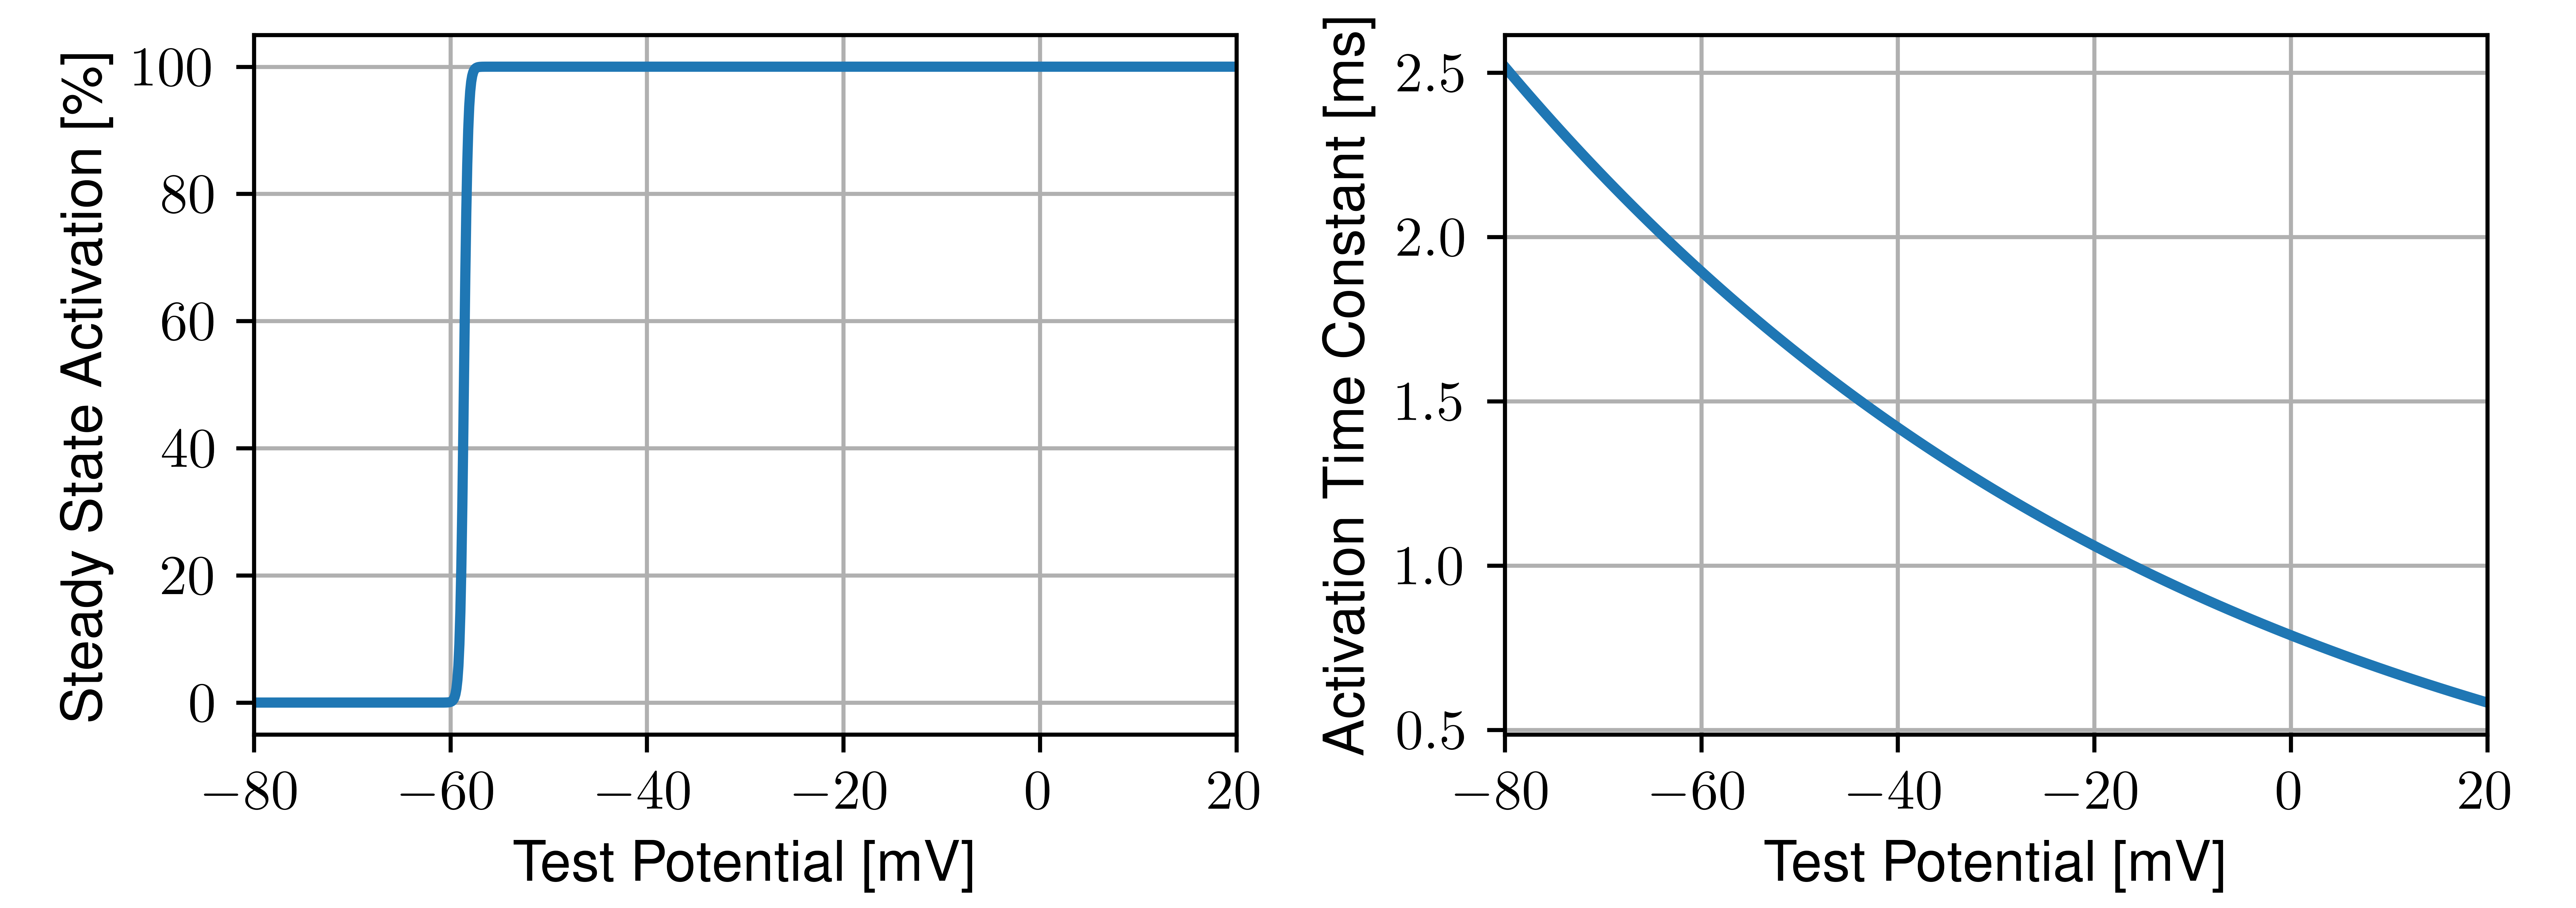
\includegraphics[width=0.8\linewidth]{../img/spiking_to_bursting/eag_wang.png}
    \caption[EAG Channel Activation Variable and Kinetics for the Wang Model]{
        \textbf{EAG Channel Activation Variable and Kinetics for the Wang Model}. \textcolor{red}{TEXT!!!}
    }
    \label{fig:spiking_to_bursting_eag_params_wang}
\end{figure}

To investigate the transition between tonic spiking and bursting mediated by the \gls{eag} channel, $g_{EAG}$ in Equation \ref{eq:current_eag} was varied from $0$ to $1$ mS/cm$^2$ to reflect potential changes in channel expression between day and night(note, that maximal conductance reflects the number of ion channels in the conductance based model. \textcolor{red}{See also Section \ref{subsec:modeling_ion_channels}}). To account for variations in the external input during the day and night, the external current was also varied. All other parameters were set to their default values as specified in Section \ref{appendix:functions_and_parameters}. Figure \ref{fig:spiking_to_bursting_wang_phase_diagram} shows how the activity, interburst interval, and number of spikes per burst depend on $g_{EAG}$ and external current for the model of thalamic relay neuron proposed by Wang \parencite{wangMultipleDynamicalModes1994}. Activity is classified as bursting, spiking, or resting and was determined as described in \textcolor{red}{Section \ref{sec:materials_and_methods}}. For the purposes of analyzing interburst interval and spike count, tonic spiking was treated as a special case of bursting, consisting of one spike per burst.

\begin{figure}[!t]
    \centering
    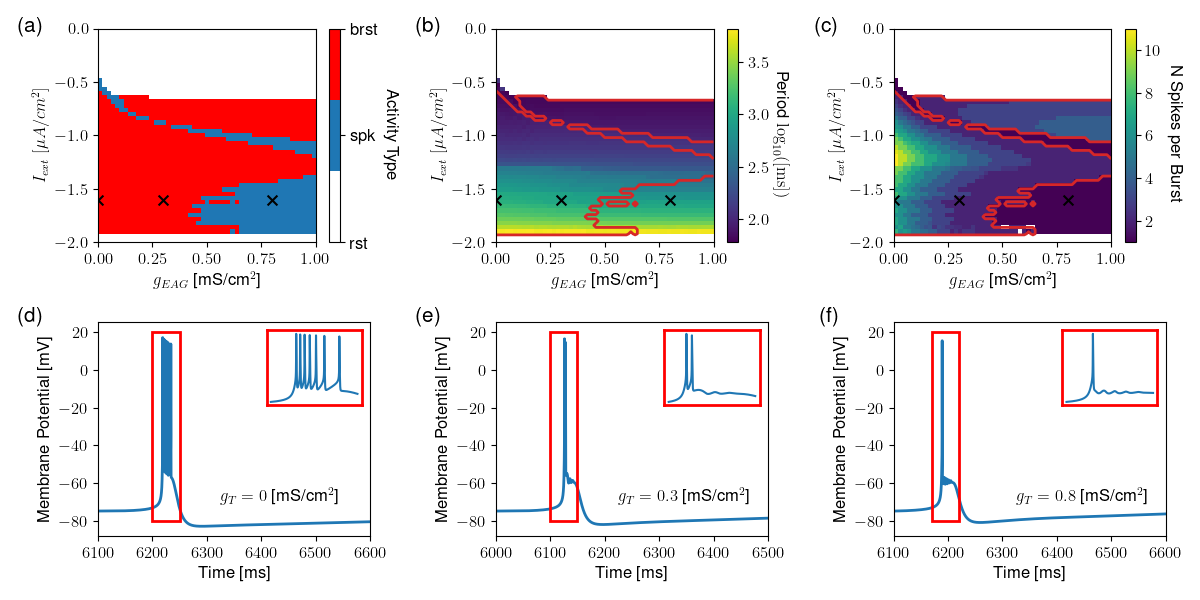
\includegraphics[width=\linewidth]{../img/spiking_to_bursting/spiking_to_bursting.png}
    \caption[Spiking-to-Bursting Transition Induced by EAG Channels in Wang model]{
        \textbf{Spiking-to-Bursting Transition Induced by EAG Channels in Wang model}. \textcolor{red}{TEXT!!! + A-F. + unit on x axis (a) Activity type; (b) Interburst period (here, tonic spiking is considered as one spike per burst), region where model showed two or more spikes per burst is outlied by red curve (corresponding to the red regions in (a); (c) number of spikes per burst); (d)-(f) examples of voltage traces in simulations. Corresponding parameter sets are denoted by "x" in (a)-(c). Insets show the closeup of the spiking, demonstrating that the number of spikes decreases with increasing $g_{EAG}$. For (d)-(f), the external input was set to $-1.6$, corresponding to the case when the model exhibits $1$Hz bursting.}
    }
    \label{fig:spiking_to_bursting_wang_phase_diagram}
\end{figure}

For fixed external input, the number of spikes mainly decreases with increasing $g_{EAG}$ and the firing pattern switches from bursting to tonic firing for a critical value of $g_{EAG}$, while the period remains relatively constant (Figure \ref{fig:spiking_to_bursting_wang_phase_diagram}a-c).
Figures \ref{fig:spiking_to_bursting_wang_phase_diagram}d-f further illustrate this effect by showing voltage traces from three representative simulations. The corresponding parameter combinations are indicated by 'x' in Figures \ref{fig:spiking_to_bursting_wang_phase_diagram}a-c.
Interestingly, there is a region in the phase space where the number of spikes increases with increasing $g_{EAG}$ (Figure \ref{fig:spiking_to_bursting_wang_phase_diagram}c, upper boundary), however, this region was not investigated within the scope of this thesis.

\textcolor{red}{The results obtained for the Goldman 1 model were qualitatively similar and are therefore not included in the main text (see Figures ??? in the Appendix)}. 

%%%%%%%%%%%%%%%%%%%%%%%%%%%%%%%%%%%%%%%%%%%%%%%%%%%%%%%%%%%%%%%%%%%%%%%%%
\subsubsection{Bifurcation analysis} \label{subsubsec:spiking_to_bursting_bifurcation}

\noindent In the previous section, it was demonstrated that the \gls{eag} channel may be responsible for termination of the burst and the emergence of tonic spiking–like behaviour in R5 neurons. This section investigates the underlying mechanisms through bifurcation analysis.

Figure \ref{fig:spiking_to_bursting_wang_bifurcation} presents the results of the bifurcation analysis for the extended Wang model with the added \gls{eag} channel. The original model generates bursting behaviour mediated by T-type Ca$^{2+}$ channels. In the model proposed by Wang \cite{wangMultipleDynamicalModes1994}, the activation gate of the T-type channel is treated as instantaneous (see Section \ref{appendix:functions_and_parameters} for details), and the slow dynamics are governed by the inactivation gate, denoted by the variable $h$. To investigate how bursting depends on this variable, $h$ was treated as a bifurcation parameter, while all other variables were allowed to evolve freely.

The analysis was performed for three representative values of $g_{EAG}$ corresponding to the '$x$' markers in Figure \ref{fig:spiking_to_bursting_wang_phase_diagram}a-c. For each value of $h$, the stable and unstable fixed points were computed using \textsc{AUTO-07p}, along with the locations of Hopf and saddle-node (\gls{sn}) bifurcations. In Figure \ref{fig:spiking_to_bursting_wang_bifurcation}, stable and unstable fixed points of the reduced system (i.e. when variable $h$ is treated as a constant) are shown as solid and dashed black lines, respectively.
Hopf bifurcations are indicated by circles, and saddle-node bifurcations by triangles. Periodic orbits were numerically continued from the Hopf bifurcations. The bursting trajectory was obtained by numerical simulations of the full system. Projection of the trajectory on the $V$-$h$ plane is overlaid as a green curve. The direction of the trajectory is indicated by the \textcolor{red}{black arrow at the bottom of the plots}.

The analysis is similar to the fast-slow decomposition discussed in Section \ref{subsec:bifurcation_analysis}. Note that plots in Figure \ref{fig:spiking_to_bursting_wang_bifurcation} extend to negative values of $h$. Although $h<0$ values do not have a physiological meaning, they are important for the completeness of the mathematical analysis.

\vspace*{0.3cm}
\noindent\textbf{EAG channel can mediate the transition from spiking to resting state}

Let us first focus on the state in which the system is spiking.
In the absence of \gls{eag} channels ($g_{\text{EAG}}=0$, Figure \ref{fig:spiking_to_bursting_wang_bifurcation} left), the trajectory is attracted by the stable limit cycle after the resting state of the reduced system (i.e. one without the $h$ variable) loses stability, causing transition of the system to the spiking state (stable limit cycle (LC), solid red lines). In the spiking state, the membrane potential provides a negative feedback to the variable $h$, corresponding to the inactivation of the corresponding gate. Consequently, the trajectory moves to the left of the $V$-$h$ plane until the stable limit cycle collides with the unstable fixed point of the reduced system. This is commonly referred to as saddle-homoclinic orbit bifurcation \parencite{izhikevichDynamicalSystemsNeuroscience2006,izhikevichNEURALEXCITABILITYSPIKING2000} (see also Section \ref{subsec:bifurcation_analysis}).

When $g_{\text{EAG}}$ is increased, the upper curve of the $V$-$h$ nullcline (black curve) is shifted to the right. This causes the saddle-homoclinic bifurcation to occur for higher values of $h$. Consequently, the system spends less time in the spiking state with increasing value of $g_{\text{EAG}}$, resulting in fewer spikes per burst (Figure \ref{fig:spiking_to_bursting_wang_bifurcation}, middle).

After $g_{\text{EAG}}$ reaches a critical point (the exact value not shown here), the trajectory does not enter the region of the $V$-$h$ plane where the limit cycle exists. Consequently, after the fixed point of the reduced system loses stability, instead of following a limit-cycle attractor, the trajectory goes back to rest via a heteroclinic orbit (Figure \ref{fig:spiking_to_bursting_wang_bifurcation} right).


\begin{figure}[!t]
    \centering
    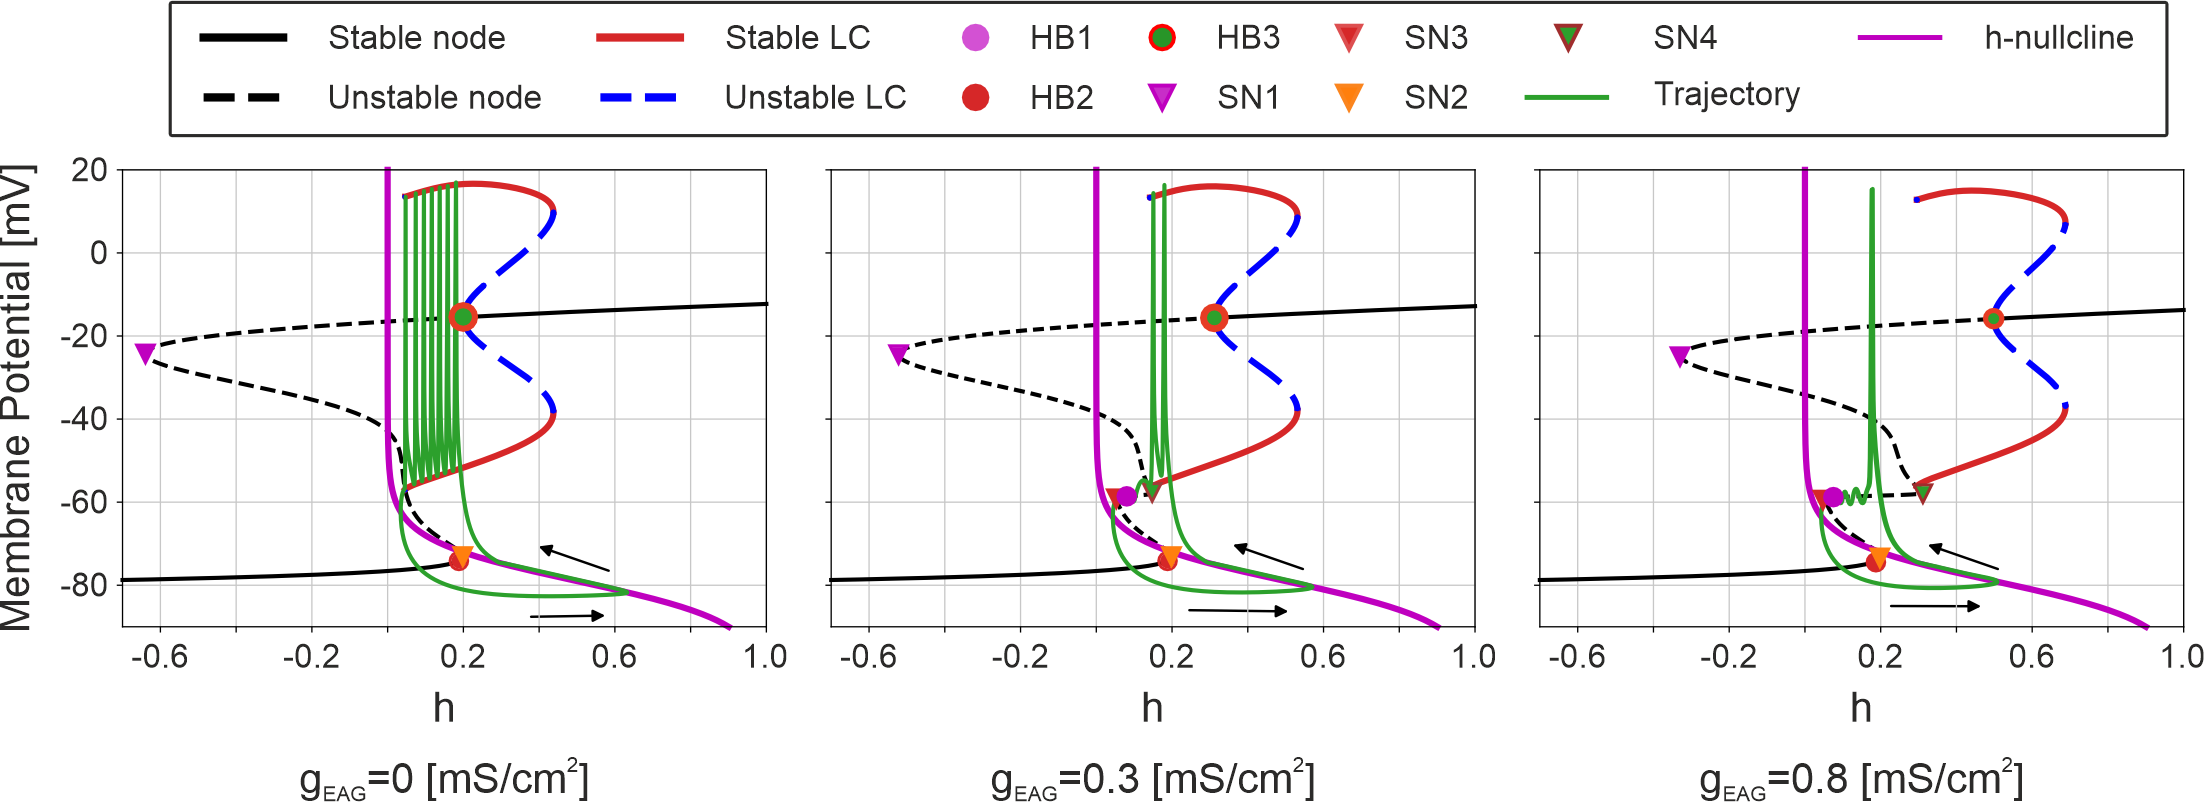
\includegraphics[width=\linewidth]{../img/spiking_to_bursting/bifurcation_wang.png}
    \caption[Transition from Spiking to Bursting via EAG channels]{
        \textbf{Transition from Spiking to Bursting via EAG channels}. \textcolor{red}{TEXT!!! + Make circles larger + A-C}
    }
    \label{fig:spiking_to_bursting_wang_bifurcation}
\end{figure}

\textcolor{red}{Look at Bifurcation in Codim-2 ???}

\textcolor{red}{Why is the curve shifting to the right? - Plot steady steady state I(V) plot for the "fast" subsystem + external current (horizontal line) for several values of $g_eag$. Their intersections will be fixed points. + two more line plots: one for I(V) of "fast" subsystem without $I_{eag}$ and another for $I_{eag}$ to visually see how I(V) is obtained from these two components}.

\vspace*{0.3cm}
\noindent\textbf{Effect of another slow variable on fast-slow decomposition}

From the perspective of fast-slow analysis, one might expect the trajectory of the full system to closely follow the manifold of stable fixed points of the reduced (or, fast) subsystem. However, the model contains an additional variable with a relatively slow timescale, associated with the \gls{hcn} channels (\textcolor{red}{see Section ??? for the corresponding parameters}). As discussed in Section \ref{subsubsec:ion_channel_contributions}, \gls{hcn} channels (referred to as "sag current" in \parencite{wangMultipleDynamicalModes1994}) are hyperpolarization-activated channels that mediate depolarizing current, thus, they contribute to dynamics at relatively low values of membrane potential.



\begin{figure}[!t]
    \centering
    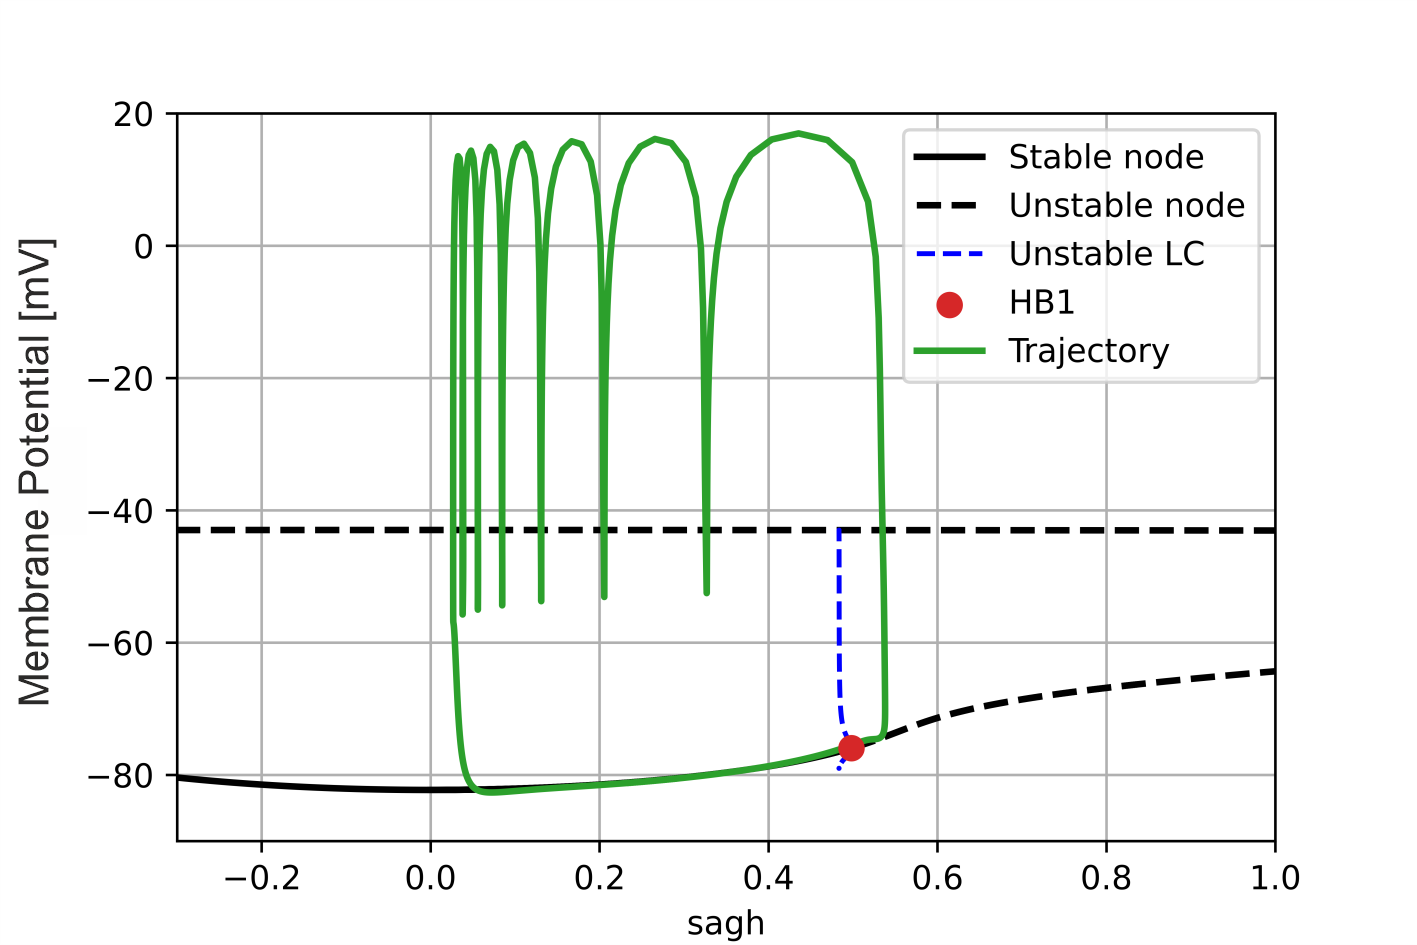
\includegraphics[width=0.6\linewidth]{../img/spiking_to_bursting/bifurcation_wang_sagh.png}
    \caption[Bifurcation Diagram - Wang Model with Sag Activation as Bifurcation Parameter]{
        \textbf{Bifurcation Diagram - Wang Model with Sag Activation as Bifurcation Parameter}. \textcolor{red}{TEXT!!!}
    }
    \label{fig:spiking_to_bursting_wang_bifurcation_sagh}
\end{figure}

Notably, \gls{hcn} channels contribute less during the spiking state. For example, at $-55$mV (approximately trough of the oscillation), the steady state activation has a value of $\sim 0.12$, decreasing to $\sim 0.06$ at $-50$mV and to $\sim 0.016$ at $-40$mV. Consequently, during the spiking state, the system behaves more like a fast-slow in contrast to the resting state. This may explain why the bifurcation diagram seems to be more accurate in the spiking state than in the resting state of the reduced ("fast") subsystem without the $h$ variable. Indeed, when the activation variable of the \gls{hcn} channel was treated as a bifurcation parameter, the resulting trajectory closely followed the manifold of stable fixed points in the reduced subsystem where the \gls{hcn} activation was held constant (Figure \ref{fig:spiking_to_bursting_wang_bifurcation_sagh}).

To summarize, the transition of interest is from the spiking to the resting state, as I hypothesize that \gls{eag} channels may terminate bursting activity. Since the above analysis effectively captures the dynamics during the spiking state, the approach remains suitable for investigating the mechanism.


\end{document}